\section{Analysis Methods of Spectral Readings}

This section explores various spectral analysis methods applied to the simulated spectral readings. Each method is evaluated for its effectiveness in measuring Carbon levels. Error is calculated using mean squared error (MSE) between the predicted and actual carbon levels in the test data.

\subsection{Calibration Layer}

All models undergo a calibration process to align their predictions with the carbon measurements. This involves a regression model between a key characteristic and the predicted values. A linear regression model is used for this purpose.

The Scipy python package is used for the fitting process\cite{virtanen_scipy_2020}, leveraging its curve fitting capabilities to refine the initial parameter estimates. All fitting problems are taken as fitting a curve f(x, p0) where p0 are the initial parameters. The fitting process iteratively adjusts these parameters to minimize the difference between the predicted and actual values, using a least-squares approach. The Levenberg-Marquardt algorithm is employed to optimize the fitting process\cite{more_levenberg-marquardt_1978}. When the fitting is bounded, Trust Region Reflective optimization \cite{branch_subspace_1999} is used.

\subsection{Peak Baseline Fitting}

Peak fitting involves using the least-squares method in identifying and quantifying the baseline and peaks in the spectral data that correspond to specific soil components \cite{gardner_use_2011}. This method is useful for extracting information about the concentration of individual elements or compounds in the soil. For effective peak fitting, the data is filtered to focus on the peak area.

The fitting function is defined as:
\begin{equation}
F_f = F_p + F_b
\end{equation}

where $F_p$ is the peak function (e.g., Gaussian) and $F_b$ is the baseline function (e.g., linear or exponential falloff).

\begin{table}[H]
\centering
\caption{Function parameterizations for peak fitting}
\label{tab:functions}
\begin{tabular}{ll}
\toprule
Function Type & Example Expression \\
\midrule
Linear & $ax + b$ \\
Exp Falloff & $a \cdot \exp(-b \cdot x) + c$ \\
Gaussian & $a \cdot \exp(-((x - b)^2)/c^2) + d$ \\
\bottomrule
\end{tabular}
\end{table}

The baseline function is subtracted from the fitted function to isolate the peak, and the area under the peak is calculated to quantify the concentration of the corresponding element or compound in the soil.

\begin{figure}[H]
\centering
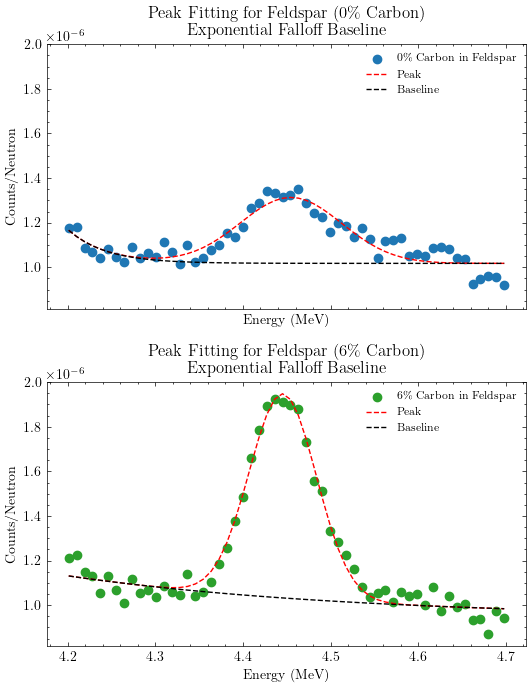
\includegraphics[width=0.8\textwidth]{../Figures/Analysis/peak_fitting_feldspar_subplots.png}
\caption{Peak fitting example showing fitted peak and baseline for feldspar spectrum}
\label{fig:peak_fitting}
\end{figure}

The final prediction is calibrated using the peak areas.

\begin{figure}[H]
\centering
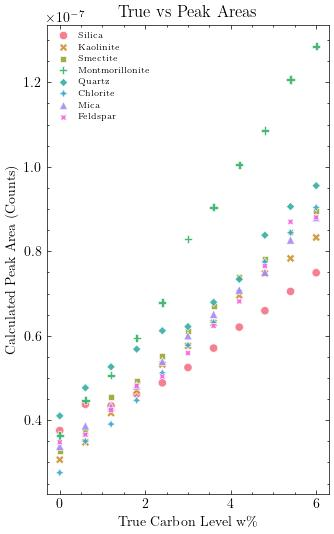
\includegraphics[width=0.8\textwidth]{../Figures/Analysis/carbon_level_vs_predicted_pf.jpg}
\caption{Peak fitting prediction results showing carbon level vs predicted values}
\label{fig:peak_predictions}
\end{figure}

\subsection{Component Fitting}

Component fitting involves modeling the spectral data as a combination of known spectral signatures of soil components. This method allows for the estimation of the concentration of multiple components in the soil based on their spectral contributions.

The combined spectral function is defined as:
\begin{equation}
F_c = \sum_{i} A_i \cdot F_i
\end{equation}

where $F_c$ is the combined spectral function, $A_i$ are the coefficients representing the concentration of each component, and $F_i$ are the spectral functions of individual components.

% \begin{figure}[H]
% \centering
% 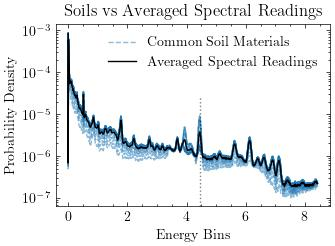
\includegraphics[width=0.8\textwidth]{../Figures/DataGeneration/CommonSoilSpectravsAverageSoilSpectrum.jpg}
% \caption{Common soil spectra vs average soil spectrum showing the spectral signatures of different soil components}
% \label{fig:common_soil_spectra}
% \end{figure}

\begin{figure}[H]
\centering
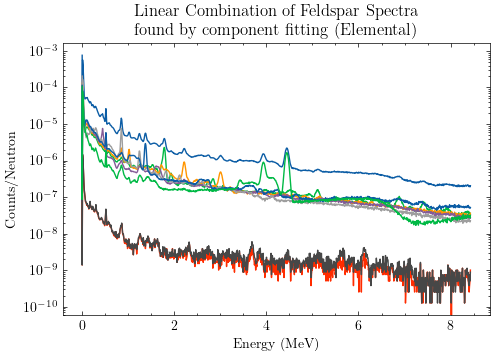
\includegraphics[width=0.8\textwidth]{../Figures/Analysis/elemental_linear_combination_feldspar.png}
\caption{Component fitting process showing linear combination of elemental spectral components for feldspar analysis}
\label{fig:elemental_component_fitting}
\end{figure}

\begin{figure}[H]
\centering
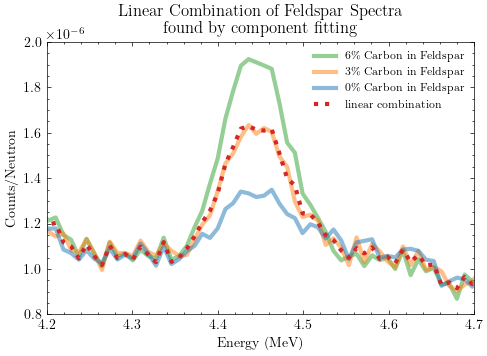
\includegraphics[width=0.8\textwidth]{../Figures/Analysis/linear_combination_feldspar.png}
\caption{Component fitting process showing linear combination of spectral components for feldspar analysis}
\label{fig:component_fitting}
\end{figure}

Components can be any known spectral signature, either from pure elemental samples \cite{kavetskiy_neutron_2023} as shown in figure \ref{fig:elemental_component_fitting} or derived from soil samples similar to the target soil \ref{fig:component_fitting}. The fitting process involves adjusting the coefficients $A_i$ to minimize the difference between the combined spectral function $F_c$ and the observed spectral data. This method also benefits from filtering of low energy signals which are generally more likely to be caused by noise.

The carbon coefficient $A_C$ is then used to estimate the Carbon level in the soil. This method is particularly useful for analyzing complex soil mixtures where multiple known components contribute to the spectral signature. This method is also generalizable to study other elements or compounds.

\begin{figure}[H]
\centering
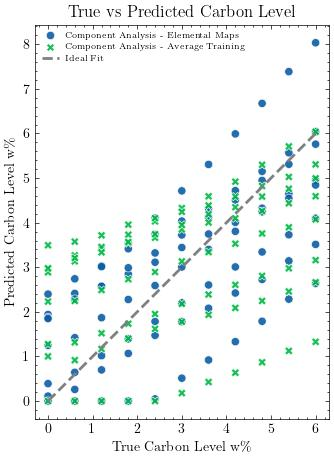
\includegraphics[width=0.8\textwidth]{../Figures/Analysis/carbon_level_vs_predicted_component_analysis.jpg}
\caption{Component fitting prediction results showing carbon level vs predicted values}
\label{fig:component_predictions}
\end{figure}

\subsection{Convex Optimization}

Convex optimization techniques can be applied to the spectral data to identify and quantify the contributions of different soil components. By formulating the problem as a convex optimization task, it is possible to find the optimal coefficients for the spectral components that minimize the difference between the observed and modeled spectra.

\begin{figure}[H]
\centering
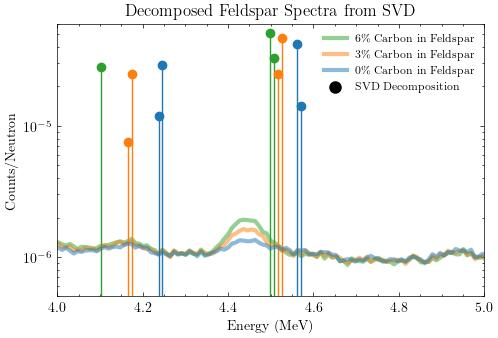
\includegraphics[width=0.8\textwidth]{../Figures/Analysis/decomposed_feldspar_svd.jpg}
\caption{Convex optimization process showing SVD decomposition of feldspar spectral data}
\label{fig:svd_decomposition}
\end{figure}

\begin{figure}[H]
\centering
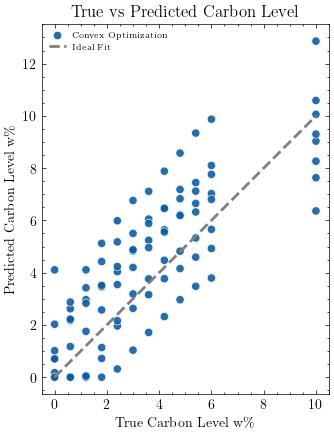
\includegraphics[width=0.8\textwidth]{../Figures/Analysis/carbon_level_vs_predicted_convex_optimization.jpg}
\caption{Convex optimization predictions showing carbon level vs predicted values using SVD}
\label{fig:svd_predictions}
\end{figure}

\subsection{Deep Learning}

Deep learning techniques, such as convolutional neural networks (CNNs), can be applied to spectral data for feature extraction and classification. These methods can learn complex relationships in the data and provide robust predictions of carbon levels based on spectral readings. The most important difference between deep learning and the previous methods is that it requires a large amount of training data to be effective. One method by Kim et al. \cite{kim_deep_2025} uses a deep learning model to predict existence, concentration and carbon peak areas.

\begin{figure}[H]
\centering
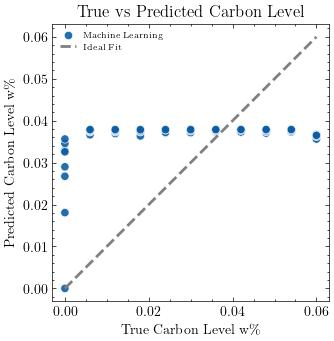
\includegraphics[width=0.8\textwidth]{../Figures/Analysis/carbon_level_vs_predicted_ml_optimization.jpg}
\caption{Deep learning prediction results showing carbon level vs predicted values using machine learning optimization}
\label{fig:ml_predictions}
\end{figure}
